\section{The Proposed Model}\label{model}
In this section, we first formally describe the Decentralized Matrix Factorization (DMF) problem. 
We then discuss a nearby user communication scheme for users to collaborate with each other. 
Next, we propose an enhanced version by applying random walk theory. 
Then, we present a privacy preserving nearby user collaboration algorithm to optimize DMF. 
We analyze the model complexity in the end.%, including communication and computation complexities.

\subsection{Preliminary}



Formally, let $\mathcal{U}$ and $\mathcal{V}$ be the user and item (POI) set with $I$ and $J$ denoting user size and item size, respectively. 
Let $(i,j)$ be an interaction between user $i \in \mathcal{U}$ and item $j \in \mathcal{V}$, and $r_{ij}$ be the rating of user $i$ on item $j$. 
Without loss of generality, we assume $r_{ij} \in [0,1]$ in this paper. 
Let $\mathcal{O}$ be the training dataset, where all the user-item ratings in it are known. 
%We also use $\mathcal{O}_u$ and $\mathcal{O}_v$ to denote the users and items in the training dataset, respectively. 

For the traditional centralized MF, it first collects all the $r_{ij} \in \mathcal{O}$, and then learns $\textbf{U}\in \mathbb{R}^{K\times{}I}$ and $\textbf{V}\in \mathbb{R}^{K\times{}J}$ using MF technique (Equation \ref{lfm}). 
Here, $\textbf{U}\in \mathbb{R}^{K\times{}I}$ and $\textbf{V}\in \mathbb{R}^{K\times{}J}$ denote the user and item latent factor matrices, with their column vectors $u_i$ and $v_j$ be the $K$-dimensional latent factors for user $i$ and item $j$, respectively.

For DMF, to guarantee the privacy of each user, we need to keep all the known ratings and latent factors on each user's end during the whole training procedure. 
To do this, we use $\textbf{U}\in \mathbb{R}^{K\times{}I}$ to denote user latent factor matrix, with each column vector $u_i$ denotes the $K$-dimensional latent factors for user $i$. 
We also use $\textbf{V}\in \mathbb{R}^{I\times{}K\times{}J}$ to denote item latent factor tensor, with $\textbf{V}^i\in \mathbb{R}^{K\times{}J}$ denotes the item latent factor matrix for user $i$, and further with $v^i_j$ denotes the $K$-dimensional latent factors for item $j$ of user $i$. 
Thus, each user $i$ only needs to store $i$'s own $K$-dimensional latent factor $u_i$, and $i$'s item latent factor matrix $\textbf{V}^i$.

Besides, users need to collaboratively learn their stored factors, i.e., $u_i$ and $\textbf{V}^i$, in DMF scenario. 
For centralized MF, all the users share the same item latent factor matrix, i.e., $\textbf{V}^i=\textbf{V}^{i'}, \forall ~ i,i' \in \mathcal{U}$. %for any two user $i$ and $i'$. 
%all the ratings of $r_{ij} \in \mathcal{O}$ will affect $\textbf{V}$ during training. 
For DMF, each user stores his $u_i$ and $\textbf{V}^i$, and they should be trained collaboratively with other users---which we call `neighbors'. 
Suppose we have a user adjacent graph $\mathcal{G}$, we use $\textbf{W}\in \mathbb{R}^{I\times{}I}$ to denote user adjacency matrix, where each element $w_{i,i'} \in [0, 1]$ denotes the degree of relationship between user $i$ and $i'$. Of course, user $i$ and $i'$ have no relationship if $w_{i,i'}=0$. 
We use $\mathcal{N}^d(i)$ to denote the $d^{st}$ order neighbors of $i$ on $\mathcal{G}$, $|\mathcal{N}^d(i)|$ as the neighbor size, and $|\mathcal{N}^D(i)|=\sum\limits_{d}^D|\mathcal{N}^d(i)|$. %with $d \in \{1,2,...,D\}$. 
Obviously, $\mathcal{N}^1(i)$ denotes the direct neighbors of $i$. %, i.e., $\mathcal{N}^1(i)=\mathcal{N}(i)$. 
Besides, to save communication cost, we use $N$ to denote the maximum number of direct neighbors of each user. 
%we use $\textbf{E}\in \{0,1\}^{I\times{}I}$ to denote the adjacency matrix, where each element $e_{i,i'} \in \{0,1\}$ denotes absence of edge between user $i$ and $i'$ or not. 
%We also use $\textbf{W}\in \mathbb{R}^{I\times{}I}$ to denote the relationship degree matrix, where each element $w_{i,i'} \subset [-1, 1]$ denotes relationship degree between user $i$ and $i'$.

DMF aims to learn $u_i$ and $\textbf{V}^i$ for each user, and the model learning procedure is performed on one's own side, e.g., cell phone and Pad.


\subsection{Nearby User Communication}
The essence of MF is that the user and item latent factors are learnt collaboratively, so should be DMF. 
Thus, \textit{which user should be communicated under DMF framework} becomes the first challenging question. 
We answer this question by first analyze the data in POI recommendation scenarios. 

\textbf{Observation.} 
%The key of optimizing DMF is how to collaborate users for updating latent factors, that is how to select collaborative users. 
%, meanwhile preserve user privacy. 
%Existing researches have shown that POI data follows power law distribution \cite{ye2011exploiting} and Gaussian distribution \cite{cho2011friendship,cheng2012fused}. 
%Inspired by the existing researches \cite{ye2011exploiting,cho2011friendship,cheng2012fused}, we find a simple way to this by data analysis. 
% We do this by first analysis the data in POI recommendation scenarios. 
Figure \ref{dataanalysis} shows the user-POI check-in distributions on two real datasets, i.e., \emph{Foursquare} and \emph{Alipay}. 
Both datasets contain user-item-check-in-location records, and we divide locations into different cities. 
We randomly select the user-item check-in records in five cities from both datasets, and plot their check-in distributions in Figure \ref{dataanalysis}, where each dot denotes a user-item check-in record. 
From it, we have the following observation: 
in POI scenarios, most users are only active in a certain city, and we call it ``location aggregation''. 
Only a few users be active in multi-cities, which is neglectable. 

% \begin{figure}[!tp]
% \centering
% 
\includegraphics[width=4cm]{figures/graph}
% %\vskip -0.1in
% \caption{User Adjacent Graph.}
% \label{graph}
% %\vskip -0.15in
% \end{figure}

\begin{figure}
\centering
\subfigure[Foursquare dataset] { 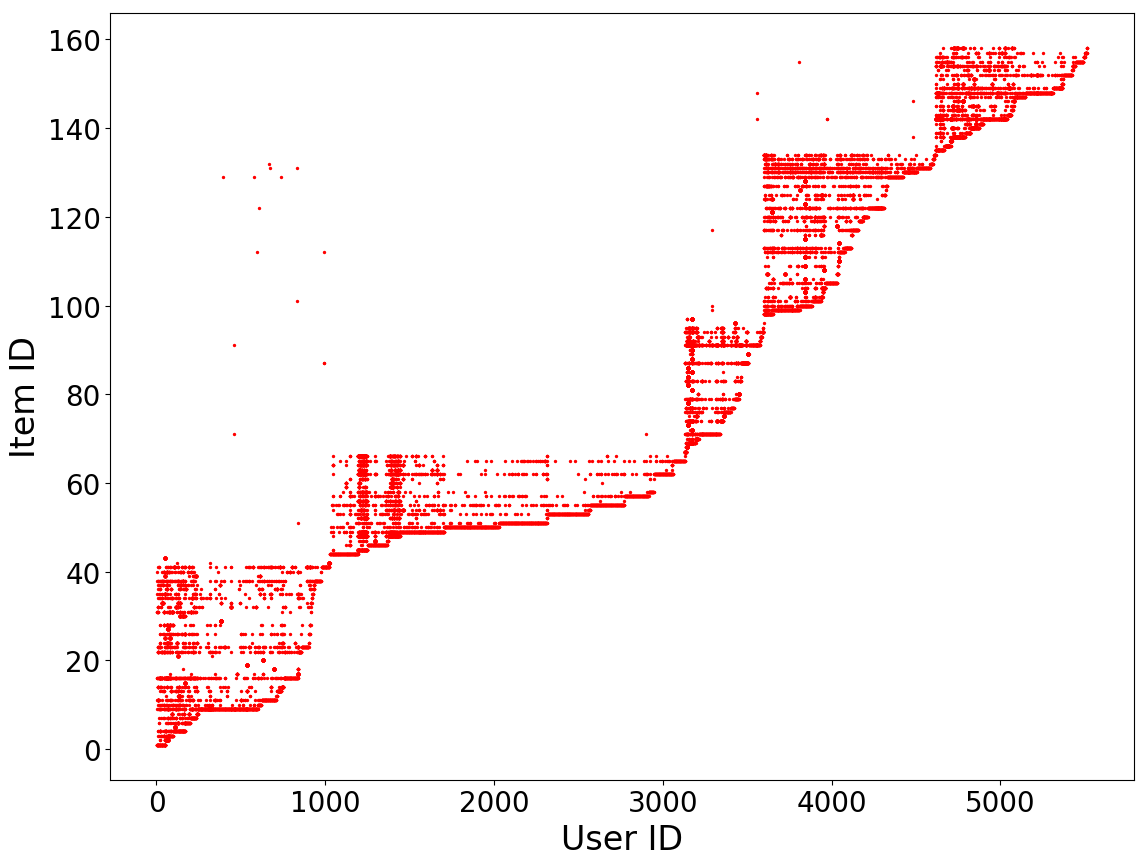
\includegraphics[width=4cm,height=3.3cm]{figures/datatist}}~~~
\subfigure [Alipay dataset]{ 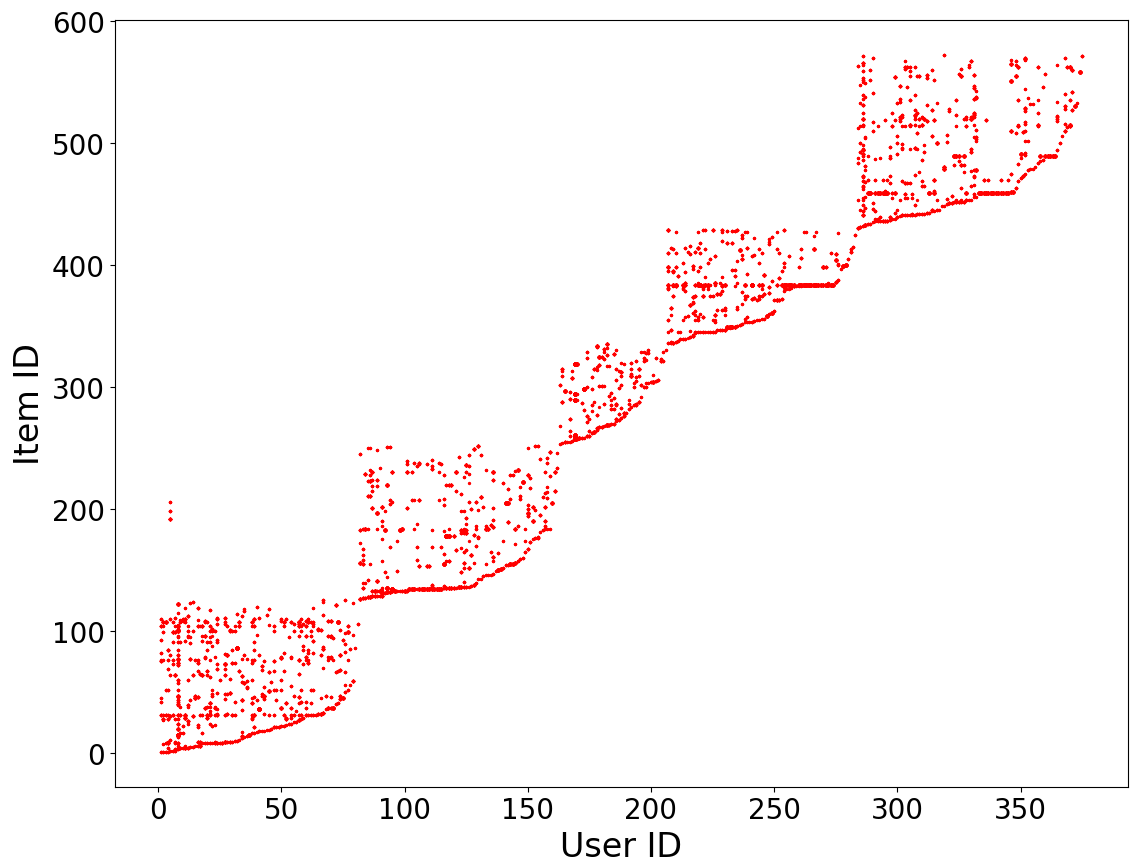
\includegraphics[width=4cm,height=3.3cm]{figures/datakb}}
\vskip -0.1in
\caption{Data analysis of Foursquare and Alipay datasets.}
\label{dataanalysis}
\vskip -0.1in
\end{figure}

\textbf{User Adjacent Graph. } 
We represent the affinities among users based on the definition of a user adjacency graph. 
It can be built using whatever information that is available, e.g., rating similarity \cite{su2009survey} and user social relationship \cite{yang2011like}. 
However, in DMF for POI recommendation scenario, users' ratings are on their own hand, and social relationship is not always available. 
Thus, we focus on using user geographical information to build user adjacent graph, similar as the existing researches \cite{ye2011exploiting,cho2011friendship,cheng2012fused}. 
%As we analysised, users in POI scenarios tend to have ``location aggregation'' property. 
% We build user adjacent graph based on their geographical information. 
Specifically, suppose %$(x^i, x^i)$ and $(x^{i'}, y^{i'})$ are the current latitude and longitude of user $i$ and $i'$ respectively, 
$d_{i,i'}$ is the distance between user $i$ and $i'$, 
the relationship degree between $i$ and $i'$ is defined as 
\begin{equation}\small
%w_{i,i'} = I^{i,i'} \cdot f((x^i, x^i),(x^{i'}, y^{i'})),
w_{i,i'} = I^{i,i'} \Large \cdot f(d_{i,i'}),
\end{equation} 
where $w_{i,i'} \in [0,1]$, $I^{i,i'}$ is the indicator function that equals to 1 if $i$ and $i'$ are in the same city and 0 otherwise, and $f(d_{i,i'})$ is a mapping function of distance and relationship degree, and the smaller the distance of $i$ and $i'$ is, the bigger their relationship degree is. 
Existing research has proposed different such mapping functions \cite{zhao2016survey}. %, which is not our focus. 
In practice, it's extremely expensive if we maintain the communications for those super-users who have a huge number of neighbors. Thus, we set $N$ to be the maximum number of neighbors each user can have. 
With nearby user communication schema, the first question is answered. 
%Moreover, the number of neighbors determinate the communication cost, and thus, in practice, the communication should only be done in a certain number of users. 
%Therefore, we use $N$ to denote the maximum number of neighbors of each user. 
%Users communicate with their neighbors on the built adjacent graph as the answer to the first question. 


\subsection{Random Walk Enhanced Nearby User Communication}

With the adjacency matrix $W$ representing the communication graph among users, \textit{how far should users communication with their neighbors} becomes the second challenging question. 
Practically, a user's decision on an item is not only affected by his direct neighbors, but also the further neighbors, e.g., the neighbors of neighbors. 
Thus, when a user $i$ rates an item $j$, this information should not only be sent to the directly neighbors of user $i$, but also his further neighbors, as shown in Figure \ref{randomwalk}. 
The challenge remains to be how far to explore the network, since there is a tradeoff between decentralization and communication/computation cost: 
the further the communication is, the more users can collaborate, meanwhile, the more communication and computation need to be done. 
We propose to solve this challenge by using random walk theory, which has been used to model trust relationship between users \cite{jamali2009trustwalker}. 


\begin{figure}[!tp]
\centering
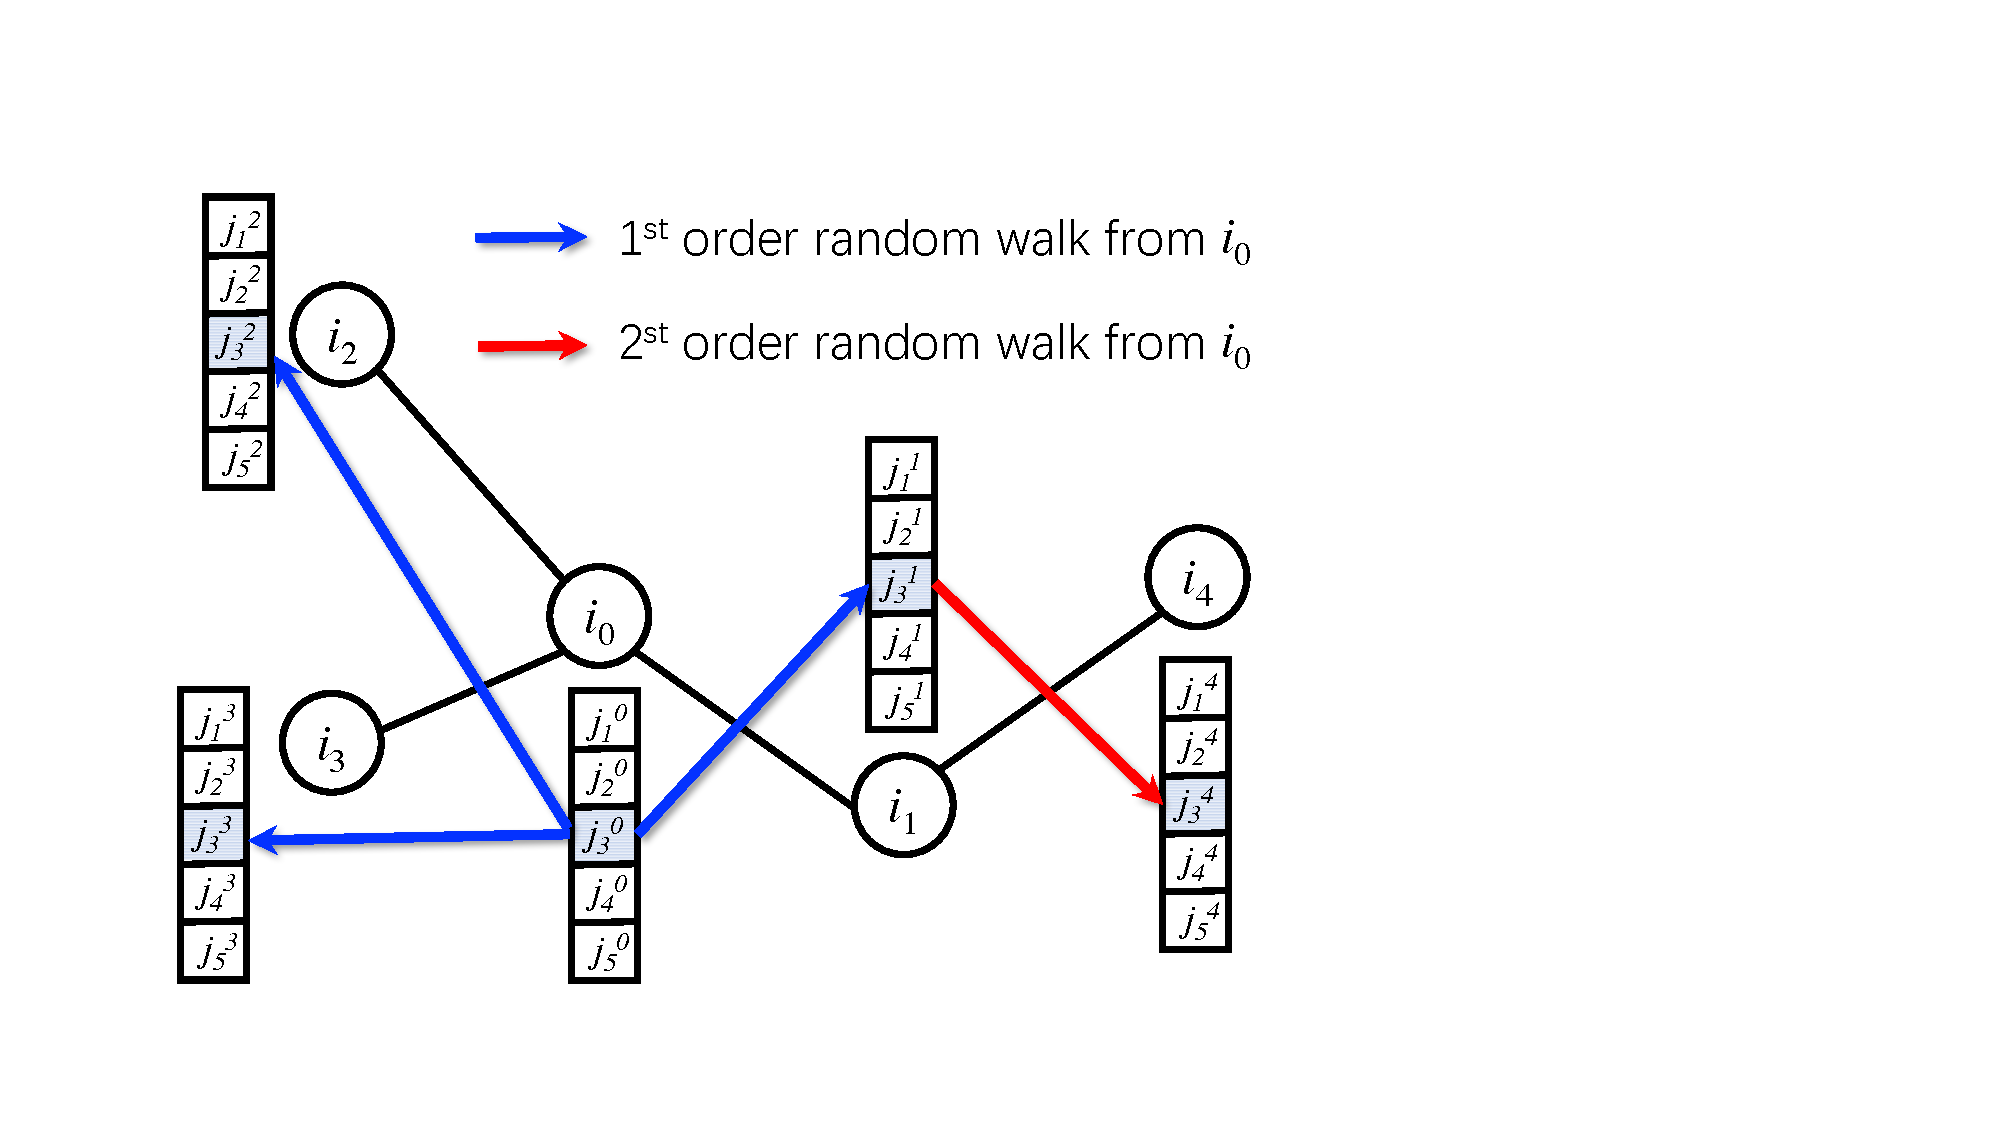
\includegraphics[width=5.5cm]{figures/randomwalk}
%\vskip -0.1in
\caption{Random walk enhanced nearby user communication. User $i_0$ communicates with his neighbors once he has an interaction with POI $j_3$. }
\label{randomwalk}
\vskip -0.15in
\end{figure}

\textbf{Random walk. }
We aim to find an intelligent way to determine how far a user communicate with his neighbors. 
% Does user $i_0$ send the gradient only to his/her $1^{st}$ order of neighbors, i.e., $i_1$, $i_2$, and $i_3$, or further to his/her $2^{st}$ order of neighbors, i.e., $i_4$? 
% We apply random walk to answer this question. 
Assuming user $i$ wants to communicate with his direct neighbors ($k \in \mathcal{N}^1(i)$), we define $n_i$ as the activity of user $i$ selecting a user from his neighbor set, and thus 
\begin{equation}\small
P(n_i = k) = \frac{w_{ik}}{\sum\limits_{i' \in \mathcal{N}^1(i)}{w_{ii'}}}. 
\end{equation} 
According to the Markov property \cite{aldous2002reversible}, the probability of user $i$ choosing his $2^{st}$ order of neighbors ($k' \in \mathcal{N}^2(i)$) is
\begin{equation}\small
%P(n_i = k') \propto P(n_i = k)  P(n_k = k') = \frac{w_{ik}}{\sum\limits_{i' \in N(i)}{w_{ii'}}}  \frac{w_{kk'}}{\sum\limits_{k' \in N(k)}{w_{kk'}}}. 
P(n_i = k') = \sum\limits_{k} P(n_i = k)  P(n_k = k') \propto \sum\limits_{k} w_{ik} w_{kk'}. 
\end{equation} 
%Inspired by the work of \cite{jamali2009trustwalker}, 
We use $D$ to denote the max distance of random walk, and generally, the adjacent matrix of $d^{st}$ order of neighbors is $W^d$. 
With random walk theory on user adjacent graph, the second question is answered. 


\subsection{DMF: Privacy Preserving Nearby User Communication.} 
The random walk based nearby user communication is an intelligent way for selecting neighbors to be communicated within POI recommendation scenarios, but the third challenging question remains: \textit{what information should users communicate with each other}, that is, how should users collaboratively learn the DMF model without leaking their data privacy. 
The original rating, of course, can clearly reflect his preference on this item. 
However, the rating itself discloses the user's privacy too much. 
Inspired by the work \cite{yan2013distributed}, we propose a privacy preserving collaborative approach for decentralized POI recommendation scenarios. 
Specifically, we suppose that for each user, the corresponding $j$-th item latent factor $v^i_j$ can be decomposed as follows: 
\begin{equation}\label{decom1}
v^i_j=p_j+q^i_j,
\end{equation} 
which implies that the latent factor of item $j$ for user $i$ is the sum between \textit{one common (global) latent factor} $p_j$ and \textit{one personal (local) latent factor} $q^i_j$, where the common factor represents the common preference of all the users while the personal factor shows the personal favor of user $i$. 
Under this assumption, the DMF model can be formulated as 
% \begin{equation}\nonumber\label{comdmf}
% \mathop { \min }\limits_{u_i,v^i_j \in \mathbb{R}^K} \mathcal{L} = \sum\limits_{i=1}^{I} l(r,u_i,v^i) + \frac{\lambda}{2} \sum\limits_{i=1}^I  ||{u_i}||_F^2 + \frac{\lambda}{2} \sum\limits_{j=1}^J||h_j||_F^2 + \frac{\lambda}{2} \sum\limits_{i=1}^I \sum\limits_{j=1}^J||h^i_j||_F^2,
% \end{equation} 
\begin{equation}\small
\label{comdmf}
\begin{split}
	\mathop { \min }\limits_{u_i,v^i_j \in \mathbb{R}^K} \mathcal{L} 
	& = \sum\limits_{i=1}^{I} l(r,u_i,v^i) + \frac{\alpha}{2} \sum\limits_{i=1}^I  ||{u_i}||_F^2 \\
	& + \frac{\beta}{2} \sum\limits_{j=1}^J||p_j||_F^2 + \frac{\gamma}{2} \sum\limits_{i=1}^I \sum\limits_{j=1}^J||q^i_j||_F^2 \\
	& ~~{\rm s.t.} ~~ v^i_j=p_j+q^i_j,
\end{split}	
\end{equation} 
where $l(r,u_i,V^i)$ can be least square loss
\begin{equation}\small
l(r,u_i,V^i)=\frac{1}{2}\sum\limits_{j=1}^{J}{\left(r_{ij} - u_i^T v^i_j\right)}^2,
\end{equation} 
which minimizes the error between real ratings and predicted ratings \cite{mnih2007probabilistic}, or listwise loss \cite{shi2010list}, as well as pairwise loss \cite{rendle2009bpr}. 
In this paper, we will take least square loss as an example. 
The last three terms in Equation (\ref{comdmf}) are regularizers to prevent overfitting. 


The factors $u_i$ and $q^i_j$ only depend on the information stored in user $i$, while the item common latent factor $p_j$ depends on the information of all the users.
Practically, in decentralized learning scenario, $p_j$ is also saved on each user's (learner's) hand, and thus, for each user $i$, $p_j$ is actually saved as $p^i_j$. Consequently, Equation (\ref{decom1}) becomes 
\begin{equation}\label{decom2}
v^i_j=p^i_j+q^i_j.
\end{equation} 
Thus, it needs one protocol for users to exchange $p^i_j$ to learn a global $p_j$. 
To solve this issue, inspired by \cite{yan2013distributed}, we propose to send the gradient of the loss $\mathcal{L}$ with respect to $p_j$, i.e., $p^i_j$ for each user $i$, to his neighbors, to help learn a global $p_j$.  
This gradient exchange method has been successfully applied in decentralized learning scenarios \cite{nedic2009distributed,yan2013distributed}, which not only guarantees model convergency, but also protects the privacy of user raw data.  
For each user $i$, the gradients of $\mathcal{L}$ with respect to $u_i$, $p^i_j$, and $q^i_j$ are:
\begin{equation}\small
\label{usergradient}
\frac{\partial \mathcal{L}}{\partial u_i} = -{\left(r_{ij} - u_i^T v^i_j\right)}v^i_j + \alpha u_{i},
\end{equation} 
\begin{equation}\small
\label{commonitemgradient}
\frac{\partial \mathcal{L}}{\partial p^i_j} = -{\left(r_{ij} - u_i^T v^i_j\right)}u_i + \beta p^i_j,
\end{equation} 
\begin{equation}\small
\label{personalitemgradient}
\frac{\partial \mathcal{L}}{\partial q^i_j} = -{\left(r_{ij} - u_i^T v^i_j\right)}u_i + \gamma q^i_j.
\end{equation} 


Based on the above gradient exchange protocol, users collaboratively learn a global $p_j$. 
Figure \ref{randomwalk} shows a demo of this protocal: $i_0$ will send ${\partial \mathcal{L}}/{\partial p^0_3}$ to his neighbors, to collaboratively learn $p_3$. 
Combining our proposed random walk enhanced nearby user communication method and gradient exchange protocol, we summarize our proposed privacy preserving DMF optimization framework for POI recommendation (Equation \ref{comdmf}) in Algorithm \ref{dmflearning}. 
As we can see that users communicate with each other by sending the common item latent factor gradients instead of raw data, i.e., ratings, which significantly reduces the possibility of information leakage. 
With the gradient exchange protocol, the third question is answered. 


From the objective function of DMF in Equation (\ref{comdmf}), we can easily make the following observations:
\begin{itemize}
\item If $\beta$ is very large, then $p_j \rightarrow 0$, and thus users will not exchange item common preferences, which means that item preference is learnt only based on their own data. 
\item If $\gamma$ is very large, then $q^i_j \rightarrow 0$, which indicates that users will not save their personal favor on items anymore. 
%Users tend to have the same latent factor for the same item, which becomes more like centralized MF. 
It will work more like centralized MF. 
\end{itemize}

The values of $\beta$ and $\gamma$ determine how well item (common and personal) preferences are learnt. We will empirically study their effects on our model performance in experiments. 

\begin{algorithm}[t]\label{dmflearning}
\caption{Random Walk Enhanced Nearby Collaborative DMF Optimization}
\KwIn {training ratings ($\mathcal{O}$), learning rate ($\theta$), user adjacency matrix ($W$), regularization strength($\alpha$, $\beta$, $\gamma$), maximum random walk distance ($D$), and maximum iterations ($T$)}
\KwOut{user latent factor ($u_i$), common item latent factor ($p^i_j$), and personal item latent factor ($q^i_j$)}

\For{$i=1$ to $I$}{
	Initialize $u_i$, $p^i_j$, and $q^i_j$
}
\For{$t=1$ to $T$}
{
	Shuffle training data $\mathcal{O}$\\
	\For{$r_{ij}$ in $\mathcal{O}$}{
		Calculate $\frac{\partial \mathcal{L}}{\partial u_i}$ based on Equation (\ref{usergradient}) \\
		Calculate $\frac{\partial \mathcal{L}}{\partial p^i_j}$ based on Equation (\ref{commonitemgradient}) \\
		Calculate $\frac{\partial \mathcal{L}}{\partial q^i_j}$ based on Equation (\ref{personalitemgradient})\\
		Update $u_i$ by $u_i \leftarrow u_i - \theta\frac{\partial \mathcal{L}}{\partial u_i}$ \\
		Update $p^i_j$ by $p^i_j \leftarrow p^i_j - \theta\frac{\partial \mathcal{L}}{\partial p^i_j}$ \\
		Update $q^i_j$ by $q^i_j \leftarrow q^i_j - \theta\frac{\partial \mathcal{L}}{\partial q^i_j}$\\
		\For{user $i'$ in $\mathcal{N}^d(i),d \in \{1,2,...,D\}$}{
			Receive $\frac{\partial \mathcal{L}}{\partial p^i_j}$ from user $i$ \\
			Update $p^{i'}_j$ by 
			$\small p^{i'}_j \leftarrow p^{i'}_j - \theta {|\mathcal{N}^d(i)|} W_{ii'}\frac{\partial \mathcal{L}}{\partial p^i_j}$
		}
	}
}
\Return $u_i$, $p^i_j$, and $q^i_j$
\end{algorithm}

%\textbf{Privacy discussion}. 
%Although the action of a user on an item is already a kind of pravicy no matter what is the rating ifself, which is the so-called implicit feedback in literature \cite{rendle2009bpr}, we claim the implicit feedback 
%As we can see from Algorithm \ref{dmflearning}, users communicate with each other by sending their gradients instead of raw data, i.e., ratings, which significantly reduces the possibility of information leakage. 

\textbf{Unobserved rating sample.} 
A universal problem in POI recommendation is that the observations are extremely sparse. 
Unless we have access to negative observations, we will probably obtain an estimator that tends to predict all the unknown $(i,j)$ as 1. 
Following the existing researches \cite{yang2011like}, we solve this problem by sampling unobserved $(i,j)$ during SGD optimization. 
Specifically, for each $r_{ij} \in \mathcal{O}$, we randomly sample $m$ missing entries $r_{{ij'}, j'=1:m}$ and treat them as negative examples, i.e., $r_{ij'}=0$. 
However, a missing entry $r_{ij'}$ can denote either $i$ does not like $j'$ or $i$ does not know the existing of $j'$. 
Therefore, we decrease the confidence of $r_{ij'}$ to $1/m$. 

%We summarize the optimization of random walk enhanced user communication and item latent tensor update procedure in Algorithm \ref{dmfrandomwalk}, and apparently, Algorithm \ref{dmfdirectneighbor} is its special case, i.e., when the random walk distance $D=1$. 
%By doing this, DMF actually share only the gradient of global item preference among connected users, instead of sharing the actual data. 


% Thus, comparing with the optimizing algorithm of DMF, the optimization of the $n^{st}$ order random walk enhanced DMF model has an additional input, i.e., the steps of random walk length ($N$), and Equation \ref{updatedelta} becomes 
% \begin{equation}
% v^{i'}_j \leftarrow v^{i'}_j - \theta \sum\limits_{n=1}^N{|\mathcal{N}(i)|} W^n_{ii'}\frac{\partial \mathcal{L}}{\partial v^i_j}
% \end{equation} 


\subsection{Complexity Analysis}
Here we analyze the communication and computation complexity of Algorithm \ref{dmflearning}. %the proposed random walk enhanced nearby collaborative DMF algorithm. 
Recall that $K$ denotes the dimension of latent factor, $N$ denotes the maximum number of direct neighbors of each user, $D$ denotes the max distance of random walk, $\mathcal{O}$ as the training data, and $|\mathcal{O}|$ as its size. 

\textbf{Communication Complexity. }
The communication cost depends on both the length of item gradient and number of neighbor to be communicated. 
Each item gradient contains $4K$ bytes information, since it is a $K$ dimensional real-valued vector. 
For user $i$, the max number of neighbors to be communicated of $D^{st}$ order random walk is $\min(|C^i|, \mathcal{N}^D(i))$, where $|C^i|$ is the number of users in the current city of $i$. 
Thus, for each $r_{ij} \in \mathcal{O}$, the communication cost is $\min(|C^i|, \mathcal{N}^D(i)) \cdot 4K$ bytes. 
It will be $|\mathcal{O}| \cdot \min(|C^i|, \mathcal{N}^D(i)) \cdot 4K$ bytes for passing the training dataset once. 
The values of $N$, $D$, and $K$ are usually small, and thus the communication cost is linear with the training data size. 

\textbf{Computation Complexity. }
The computation cost mainly relies on two parts, (1) calculating gradients, i.e., Line $7-9$ in Algorithm \ref{dmflearning}, and (2) updating user and item latent factors, i.e., Line $10-12,15$ in Algorithm \ref{dmflearning}. 
For a single pass of the training data, the time complexity of (1) is $|\mathcal{O}| \cdot K$, and the time complexity of (2) is $|\mathcal{O}| \cdot \min(|C^i|, \mathcal{N}^D(i)) \cdot K$. 
Therefore, the total computational complexity in one iteration is $|\mathcal{O}| \cdot \min(|C^i|, \mathcal{N}^D(i)) \cdot K$. 
The values of $N$, $D$, and $K$ are usually small, and thus the time complexity is linear with the training data size. 

The above communication and computation complexity analysis shows that our proposed approach is very efficient and can scale to very large datasets. 

%\subsection{Generalization}
%Our proposed decentralized MF framework has good extensibility, which can be easily modified to adapt to scenarios where other kinds of information are available. For example, when social or contextual information ...